\documentclass[11pt]{beamer}
\usepackage{verbatim}
\usepackage{amsmath}
\usepackage{amsthm}
\usepackage{graphics}
\usepackage{multicol}
\usepackage{color}
\usepackage{stmaryrd}
\usefonttheme[onlymath]{serif}

\title{Progess Report 5}
\date{\today}
\author{Xie Li}
\begin{document}
\maketitle

\begin{frame}\frametitle{Overview of the Progress}
\begin{itemize}
\item Discussion with Liyong about the algorithm.
\item Continue the development of the tool with Weizhi, implemented  data structure and basic operations of \texttt{Automaton}.
\item Integrate \textsc{Z3} and \textsc{Spot} to CMake.
\item Refine the previous implementation to make it more abstract.
\item Reading paper: 

[CAV'16] Array Fold Logic.

The report will be given tommorrow.

\end{itemize}

\end{frame}

\begin{frame}\frametitle{Algorithm}
\begin{itemize}
\item Currently focus on simple LTL properties: 
\[\textbf{F}p, \textbf{G}p, \textbf{FG}p, \textbf{GF}p\]
and their combinations.

\item Currently implementing: verify these properties while generating the path conditions.
\end{itemize}

\end{frame}
\begin{frame}\frametitle{Progress of Developing}

\textbf{Current Framework of the Tool:}
\begin{figure}
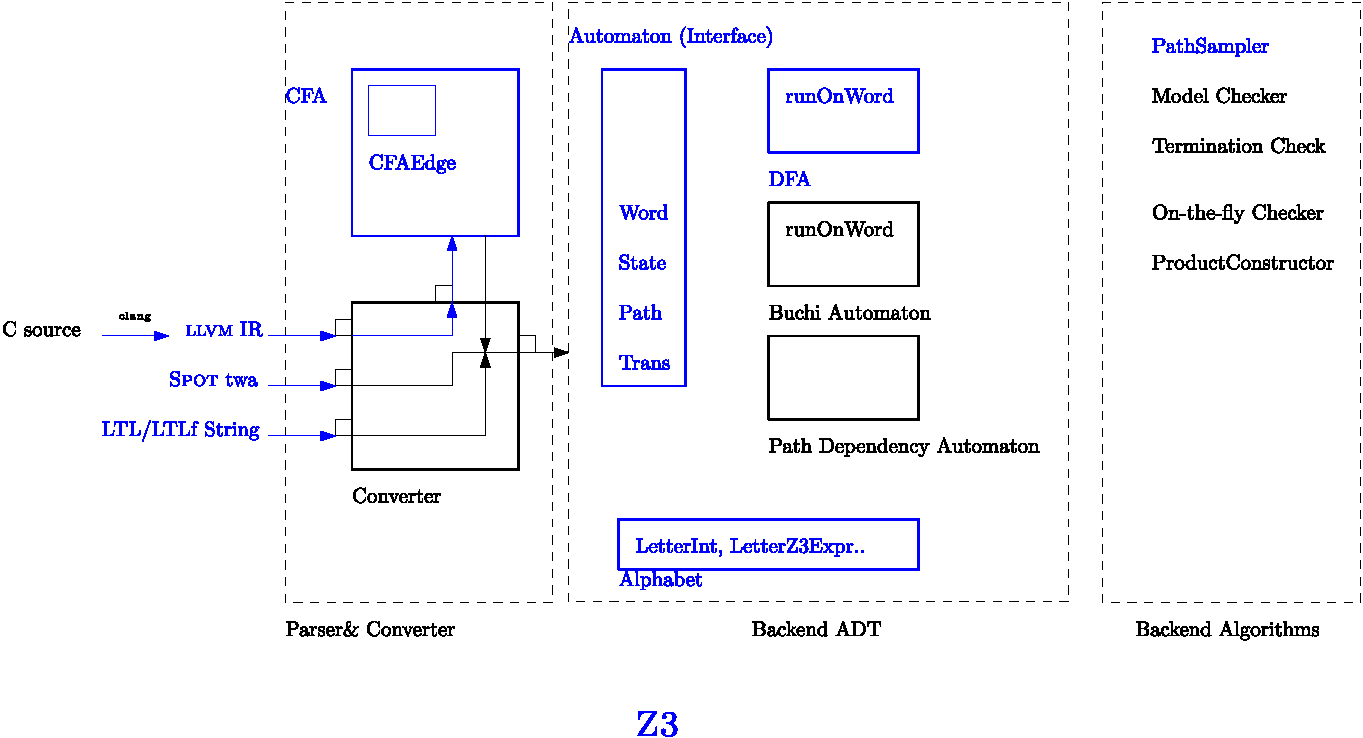
\includegraphics[scale=0.5]{tool.pdf}
\end{figure}

\end{frame}

\begin{frame}\frametitle{Future Work}
\begin{itemize}

\item Implement algorithms.
\item Continue to implement the converter for different data structure and data format.
\item Survey on more algorithms and techniques. Read more papers and report.
\end{itemize}
\end{frame}

\end{document}